\documentclass[11pt]{article}
\usepackage[margin=1in]{geometry}
\usepackage{mathpazo}
\usepackage{amsmath,amssymb}
\usepackage{microtype}
\usepackage{booktabs}
\usepackage{graphicx}
\usepackage[dvipsnames]{xcolor}
\usepackage{tikz}
\usetikzlibrary{positioning,arrows.meta,calc,fit,backgrounds}
\usepackage[most]{tcolorbox}
\usepackage{enumitem}
\usepackage{listings}
\usepackage[font=small,labelfont=bf]{caption}
\usepackage{hyperref}
\hypersetup{colorlinks=true,linkcolor=MidnightBlue,citecolor=MidnightBlue,urlcolor=MidnightBlue}
\usepackage{cleveref}
\urlstyle{tt}
\def\UrlBreaks{\do\_\do/\do.}
\newcommand{\file}[1]{\nolinkurl{#1}}
\newcommand{\code}[1]{\texttt{#1}}
\newcommand{\mhh}{m_{hh}}
\newcommand{\bw}{\boldsymbol{\omega}}
\newcommand{\bp}{\boldsymbol{p}}
\newcommand{\bx}{\boldsymbol{x}}
\newcommand{\data}{\mathcal{D}}

\definecolor{trainable}{HTML}{1B6CA8}
\definecolor{physics}{HTML}{2E933C}
\definecolor{datac}{HTML}{7B4EA3}
\definecolor{warn}{HTML}{C0392B}

\newtcolorbox{keyidea}[1][]{enhanced,breakable,colback=physics!6,colframe=physics!70!black,
  fonttitle=\bfseries,title={#1},boxrule=0.6pt,arc=2pt,left=6pt,right=6pt}
\newtcolorbox{aside}[1][]{enhanced,breakable,colback=trainable!5,colframe=trainable!70!black,
  fonttitle=\bfseries,title={#1},boxrule=0.6pt,arc=2pt,left=6pt,right=6pt}
\newtcolorbox{assume}[1][]{enhanced,breakable,colback=datac!5,colframe=datac!70!black,
  fonttitle=\bfseries,title={#1},boxrule=0.6pt,arc=2pt,left=6pt,right=6pt}
\newtcolorbox{watch}[1][]{enhanced,breakable,colback=warn!5,colframe=warn!70!black,
  fonttitle=\bfseries,title={#1},boxrule=0.6pt,arc=2pt,left=6pt,right=6pt}
\setlist{itemsep=2pt,topsep=3pt}
\setlength{\emergencystretch}{3em}

\lstset{language=Python, basicstyle=\ttfamily\small, columns=fullflexible,
  keepspaces=true, commentstyle=\color{physics!70!black}\itshape,
  keywordstyle=\color{trainable!90!black}\bfseries, stringstyle=\color{datac},
  showstringspaces=false, frame=single, rulecolor=\color{gray!40},
  backgroundcolor=\color{gray!3}, xleftmargin=4pt, xrightmargin=4pt,
  aboveskip=6pt, belowskip=6pt}

\newcommand{\what}{\hat{\boldsymbol{\omega}}}

\title{\textbf{Why is the Bayesian network so confident?}\\[4pt]
\large Diagnosis, and a plan for a Bayesian uncertainty for \texttt{HEFTNet}\\
\large from a mixture of Laplace approximations\\[4pt]
\normalsize For approval before any code is written}
\date{October 31, 2026 (revised: mixture of Laplace approximations)}

\begin{document}
\maketitle

\begin{abstract}
\noindent
The full-data Bayesian network (\file{runs/BNN_poisson_full}) gives a posterior mean
almost as accurate as the fine-tuned ensemble, but a posterior standard deviation of only
0.5\% of the POWHEG noise, so that its pulls have a standard deviation of 1.37 just above
threshold. Before a Bayesian result appears in a paper, we must know \emph{why}. A
posterior that is too narrow can have four causes: (A) the chain has not explored the mode
it sits in, (B) it has not visited the other modes, (C) the likelihood claims the network
describes POWHEG better than it does, and (D) the prior. A and B are failures of the
computation; C and D are choices in the model. The evidence in hand points strongly to A,
and to B and C. We therefore replace the Markov chain by an approximation that suffers from
neither A nor B: the posterior is approximated by a \emph{mixture of Gaussians}, one about
each of the 20 networks of the fine-tuned ensemble, each obtained by linearising the
network about that point (the linearised Laplace approximation of MacKay). It needs no
sampling, takes of order an hour on the 5090, and gives the within-mode and between-mode
uncertainties separately. Cause C is handled, as in the appendix, by a model-error term.
Nothing is written until you approve; the decisions are collected in
\cref{sec:decisions}.
\end{abstract}

\begin{keyidea}[The message for the paper]
Bayes' theorem is not on trial. The posterior answers a precisely posed question: given
\emph{this} network, \emph{this} prior and a likelihood that says the POWHEG noise is the
only discrepancy, how well are the network's parameters, and hence its predictions,
determined? If the computation is done correctly, that answer is right; if the predictions
are then too confident, the fault lies in the question, namely in the likelihood, which
ignores the error of the model itself. The plan is designed to end in the statement: ``the
posterior, approximated by a mixture of Laplace approximations about the ensemble networks,
together with a model-discrepancy term, gives calibrated uncertainties''; or in a clear
account of what prevents it. The Markov chain results are then explained, not hidden: a
single chain of this length cannot sample a 3,944-dimensional posterior with this
geometry.
\end{keyidea}

\tableofcontents

% ===========================================================================
\section{What we observed}
\label{sec:observed}

\begin{table}[h]
\centering
\small
\begin{tabular}{lccc}
\toprule
 & median $s/\sigma_k$ & s.d.\ of pull, 255--555 GeV & s.d.\ of pull, $> 555$ GeV \\
\midrule
Bayesian network (\file{BNN_poisson_full}) & 0.005 & 1.37 & 1.06 \\
fine-tuned ensemble, bootstrap & 0.056 & 1.15 & 1.04 \\
\quad + model error, $a(m_{hh})$ & 0.32 & 1.02 & 1.00 \\
\bottomrule
\end{tabular}
\caption{Calibration on the 1,000 test spectra (from the draft appendix).}
\label{tab:obs}
\end{table}

The earlier runs (\file{docs/bnn/bnn_run1.pdf} to \file{bnn_run3.pdf}: a Laplace
likelihood; the Gaussian likelihood with known variances on 10\% of the data, with fewer
and then more leapfrog steps) showed the same symptom, the first of them a chain that
hardly moved at all. The full-data run is the best of them, and it is the one analysed
here. The run: Gaussian likelihood with the known POWHEG variances (the \code{poisson} option),
hierarchical Gaussian prior with 16 Gibbs-sampled precisions \cite{Neal:1996}, warm start from
\file{runs/L1Loss}, 1,000 warm-up iterations, 1,000 samples, 800 leapfrog steps,
acceptance rate 0.72, final step size $\varepsilon \approx 7.7\times10^{-4}$. The effective
sample size of the two monitored predictions is about 135. The posterior mean differs from
the ensemble mean by a median of 0.8 ensemble standard deviations: a perfectly sensible
central value, with an implausibly narrow band around it.

% ===========================================================================
\section{Four ways a posterior can be too narrow}
\label{sec:four}

\begin{figure}[h]
\centering
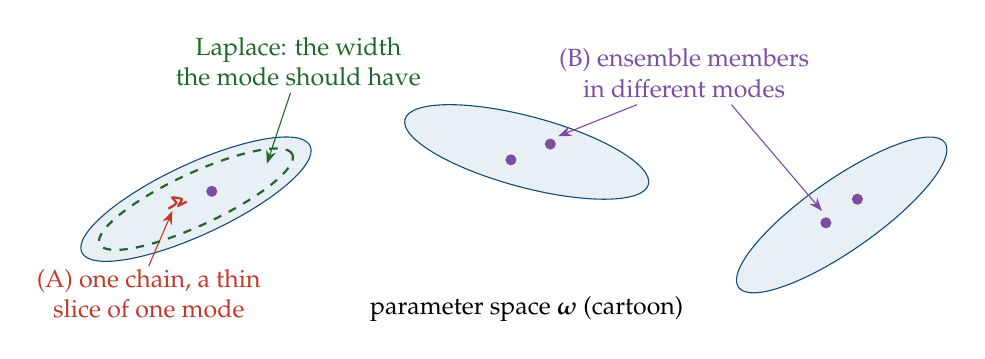
\begin{tikzpicture}[scale=1.0,>=Stealth]
  % modes
  \foreach \x/\y/\r in {0/0/25, 4.2/0.6/-15, 8.2/-0.2/35}{
    \fill[trainable!10] (\x,\y) ellipse [x radius=1.6, y radius=0.45, rotate=\r];
    \draw[trainable!70!black] (\x,\y) ellipse [x radius=1.6, y radius=0.45, rotate=\r];
  }
  % stuck chain in mode 1
  \draw[warn,thick] plot[smooth] coordinates {(-0.35,-0.12) (-0.25,-0.05) (-0.3,0.02) (-0.18,0.0) (-0.22,-0.08) (-0.12,-0.03)};
  \node[warn,font=\small,align=center] at (-0.6,-1.2) {(A) one chain, a thin\\slice of one mode};
  \draw[warn,->] (-0.6,-0.85) -- (-0.3,-0.15);
  % laplace ellipse
  \draw[physics!70!black,dashed,thick] (0,0) ellipse [x radius=1.35, y radius=0.33, rotate=25];
  \node[physics!70!black,font=\small,align=center] at (1.3,1.75) {Laplace: the width\\the mode should have};
  \draw[physics!70!black,->] (1.2,1.35) -- (0.9,0.45);
  % ensemble points
  \foreach \x/\y in {0.2/0.1, 4.0/0.5, 4.5/0.7, 8.0/-0.3, 8.4/0.0}{\fill[datac] (\x,\y) circle (2pt);}
  \node[datac,font=\small,align=center] at (6.2,1.6) {(B) ensemble members\\in different modes};
  \draw[datac,->] (5.6,1.2) -- (4.6,0.8);
  \draw[datac,->] (6.8,1.2) -- (7.95,-0.15);
  \node[font=\small] at (4.2,-1.4) {parameter space $\bw$ (cartoon)};
\end{tikzpicture}
\caption{Cartoon of the posterior: several separated modes (blue). A chain that mixes
poorly covers a thin slice of one mode (red); the linearised Laplace approximation gives the
width a well-sampled mode should have (green); ensemble members sit in different modes
(purple). Causes C and D change the shape of the ellipses themselves.}
\label{fig:cartoon}
\end{figure}

\begin{description}[leftmargin=1.2em]
  \item[A. Poor sampling within a mode.] HMC moves along stiff and soft directions alike
    with one step size, set by the stiffest. If the mass matrix does not equalise the
    curvatures, the soft directions are explored by a slow random walk, and a chain of
    $10^3$ iterations sees only a fraction of their width.
  \item[B. Modes not visited.] Networks have many separated modes (equally good solutions
    that are not related by a symmetry). A single chain stays in one
    \cite{Izmailov:2021}. The seeds ensemble
    shows that about 80\% of the ensemble variance is of this kind.
  \item[C. An over-confident likelihood.] The likelihood $\prod_k
    \mathcal{N}(t_k; f_k, \sigma_k^2)$ asserts that the network can represent the true
    cross section exactly and that the POWHEG noise is the only discrepancy. The model-error
    study says otherwise: on data not used in the training, a further variance
    $a\,\sigma_k^2$ with $a = 0.1$--0.75 is needed.
  \item[D. The prior.] With $2.7\times10^5$ training rows the likelihood dominates every
    direction that affects the predictions at points like the training points; the prior
    mainly controls the directions the data leave free, which hardly affect the predictions.
    A factor of ten from the prior would be surprising, but it is cheap to check.
\end{description}

\begin{watch}[A and B are different questions]
Even a perfect sampler need not make the posterior as wide as the ensemble. Whether the
modes of \cref{fig:cartoon} contribute to the posterior depends on their probability
\emph{mass}: if one mode has a mass $e^{100}$ times that of the others, the posterior is
that mode, and the ensemble spread, although a fair description of the variability of the
\emph{training procedure}, is not part of the Bayesian answer. We return to this when
choosing the weights of the mixture (\cref{sec:weights}).
\end{watch}

% ===========================================================================
\section{Evidence already in hand}
\label{sec:evidence}

\subsection{An identity: the effective number of parameters}

For a model linear in its parameters, $f = J\bw$, with Gaussian noise of known variances
$\sigma_k^2$ and a Gaussian prior of precision $A$, the posterior covariance is
$\Sigma = (J^{\mathsf T} W J + A)^{-1}$ with $W = \mathrm{diag}(1/\sigma_k^2)$, and
\begin{equation}
  \sum_{k=1}^{N} \frac{\mathrm{Var}_\text{post}[f_k]}{\sigma_k^2}
  = \mathrm{tr}\big(J^{\mathsf T} W J\, \Sigma\big)
  = \sum_i \frac{\lambda_i}{\lambda_i + \alpha_i} \equiv \gamma ,
  \label{eq:gamma}
\end{equation}
where, for a prior $A = \alpha I$, the $\lambda_i$ are the eigenvalues of
$J^{\mathsf T}WJ$. This is MacKay's ``number of well-determined parameters''
\cite{MacKay:1992}: each direction pinned down by the data contributes one, each direction
left to the prior contributes nothing, so $0 \le \gamma \le p$. Near a mode a network is
approximately linear in its parameters, so \cref{eq:gamma} applies approximately: the
sum over the training rows of $s_k^2/\sigma_k^2$, with $s_k$ the posterior standard
deviation of the prediction, counts the well-determined parameters.

\begin{keyidea}[What the run says]
Estimating the sum as $N$ times the average of $s_k^2/\sigma_k^2$ over the test spectra
(right panel of \cref{fig:evidence}), the Bayesian run gives $\gamma \approx 50$ out of
$p = 3{,}944$ parameters. For a network that represents 23 functions of $m_{hh}$ well
enough to give $\chi^2/N \approx 1.1$ on 80 bins over a 5-dimensional parameter space,
that is far too few. The fine-tuned ensembles, which are not posteriors, give 3,100--4,800:
the order of magnitude a well-determined network of this size should have. A correctly
sampled single mode is therefore expected to give a width of order the ensemble spread,
roughly ten times what the chain reports. This points to cause A.
\end{keyidea}

\begin{figure}[h]
\centering
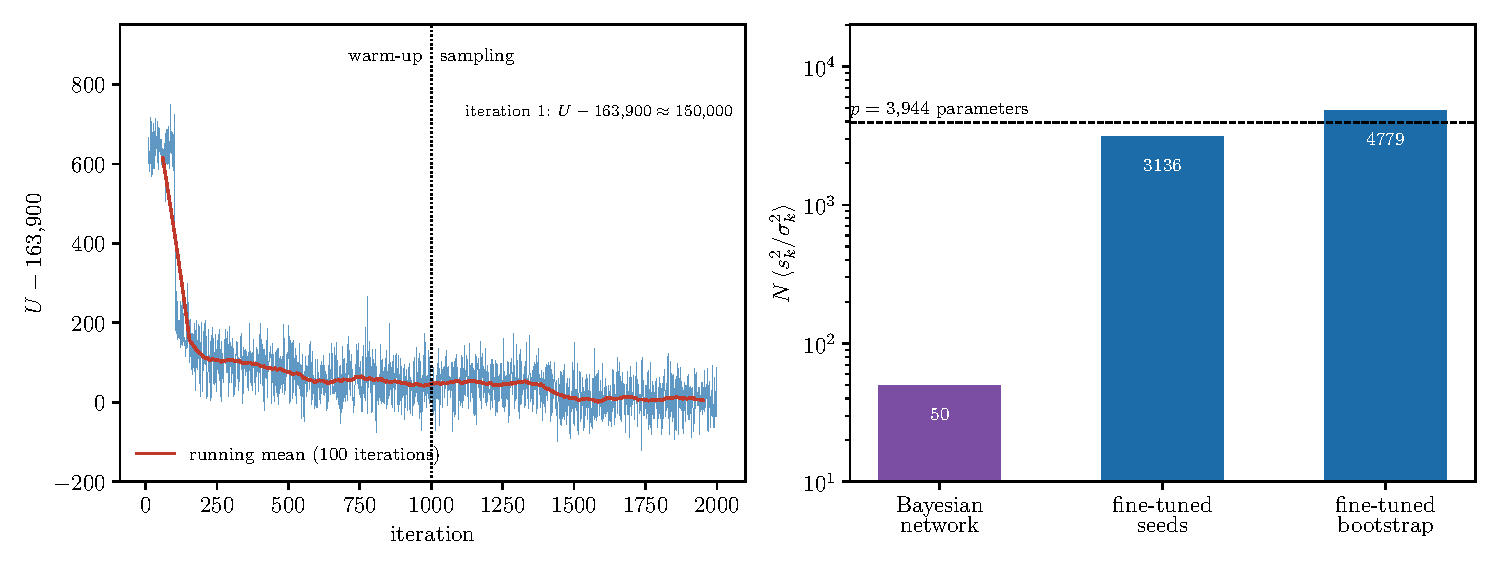
\includegraphics[width=\textwidth]{fig_evidence.pdf}
\caption{Left: the potential energy $U$ of \file{BNN_poisson_full} from iteration 10 on (it
starts 150,000 higher, at the L1 solution, and falls within ten iterations). It falls in
steps, at the first mass-matrix updates, and is still drifting downwards during sampling,
by about 100 over 1,800 iterations, two standard deviations of its fluctuations. Right:
$N\langle s_k^2/\sigma_k^2\rangle$, an estimate of the number of well-determined
parameters, \cref{eq:gamma}, for the Bayesian network and, for comparison, for the two
fine-tuned ensembles.}
\label{fig:evidence}
\end{figure}

\subsection{The chain was still relaxing}

The left panel of \cref{fig:evidence} shows that the chain reached the $\chi^2$ region
within ten iterations, sat nearly still for the first 150 iterations (the step size was
$\sim\!10^{-7}$ until the first mass-matrix updates), and has been drifting slowly
downhill ever since. A drift that persists through the whole sampling phase means the chain
has not reached its stationary distribution; samples drawn while it relaxes are too tightly
clustered. Note that the size of the fluctuations of $U$ (standard deviation 45, close to
$\sqrt{p/2} = 44$ expected for a $p$-dimensional Gaussian) is \emph{not} evidence of
good mixing: they are dominated by the stiff directions, which mix fast, and by the Gibbs
updates of the 16 precisions.

\subsection{The step size}

The leapfrog integrator \cite{Neal:2011} is stable only if $\varepsilon \lesssim 2/\sqrt{\lambda_\text{max}}$,
where $\lambda_\text{max}$ is the largest curvature of $U$ in the coordinates set by the
mass matrix. If the diagonal mass matrix had equalised the curvatures, $\varepsilon$ would
be of order $p^{-1/4} \approx 0.1$ and a few tens of leapfrog steps would cross a mode. The
tuned $\varepsilon \approx 8\times10^{-4}$ implies a remaining curvature ratio of order
$10^6$: strong correlations between parameters, which a diagonal mass matrix cannot remove.
800 leapfrog steps then move the soft directions by only a fraction of their width per
iteration. There is a further trap: the mass matrix is estimated from the spread of the
chain during warm-up, so a direction that barely moves gets a small estimated variance and
moves even less in the next window.

\subsection{The likelihood is too confident}

At the end of the run, $U \approx 163{,}900$. The prior term
$\tfrac12\sum_i\tau_{g(i)}\omega_i^2$ is about $p/2 \approx 2{,}000$, the rest is the
likelihood term $\tfrac12\sum_k r_k^2$: $\chi^2 \approx 1.18$ per training row (with the
training variances, which include the one-event term and are therefore, if anything,
generous), where a correct
noise model with $\gamma \ll N$ well-determined parameters should give $1 - \gamma/N
\approx 1$. The training data themselves therefore say what the test spectra said: the
residual variance is about 20\% larger than the POWHEG noise, on average over $m_{hh}$
(cause C).


\subsection{The diagnosis in brief}

\begin{keyidea}[Why the first attempts gave implausibly small uncertainties]
\begin{enumerate}
  \item \textbf{A, poor sampling within a mode} (the main cause): the chain's widths
    correspond to about 50 well-determined parameters, where a few thousand are expected;
    the step size shows that the diagonal mass matrix leaves curvature ratios of order
    $10^6$; and the chain was still relaxing when sampling stopped.
  \item \textbf{B, one mode}: a single chain started from one network stays near it, while
    80\% of the ensemble variance is between different solutions.
  \item \textbf{C, an over-confident likelihood}: $\chi^2 \approx 1.18$ per training row,
    and the held-out model-error term of the appendix.
  \item \textbf{D, the prior}: not implicated by anything we have seen, but untested; the
    plan tests it at no extra cost (\cref{sec:prior}).
\end{enumerate}
Making the chain correct would require a dense mass matrix and several much longer chains.
The mixture of Laplace approximations removes A and B by construction, at a small fraction
of the cost, and makes C explicit.
\end{keyidea}

% ===========================================================================
\section{The mixture of Laplace approximations}
\label{sec:mola}

\subsection{One network: the linearised Laplace approximation}

Near a network $\what_m$ of the ensemble, replace the network by its linearisation,
\begin{equation}
  f(\bx;\bw) \approx f(\bx;\what_m) + \boldsymbol{j}_m(\bx)^{\mathsf T}(\bw - \what_m),
  \qquad \boldsymbol{j}_m(\bx) = \frac{\partial f(\bx;\bw)}{\partial\bw}\Big|_{\what_m} .
  \label{eq:lin}
\end{equation}
With a Gaussian likelihood of known variances $\sigma_k^2$ and the Gaussian prior of
precisions $\tau_g$, the posterior of the linearised model is Gaussian, with precision
\begin{equation}
  H_m = \sum_{k=1}^{N} \frac{\boldsymbol{j}_{m,k}\, \boldsymbol{j}_{m,k}^{\mathsf T}}{\sigma_k^2}
      + \mathrm{diag}(\tau_{g(i)}) \equiv G_m + T ,
  \label{eq:H}
\end{equation}
where $\boldsymbol{j}_{m,k} = \boldsymbol{j}_m(\bx_k)$ and the sum runs over the training
rows. $G_m$ is the generalised Gauss--Newton matrix; it is the curvature of the $\chi^2$
without the term proportional to the residuals, and is always positive. The prediction at
any point $\bx$ is then Gaussian, with mean and variance
\begin{equation}
  \mu_m(\bx) = f(\bx;\what_m), \qquad
  v_m(\bx) = \boldsymbol{j}_m(\bx)^{\mathsf T} H_m^{-1} \boldsymbol{j}_m(\bx) .
  \label{eq:glm}
\end{equation}
This is MacKay's approach to Bayesian networks \cite{MacKay:1992}, known today as the
linearised Laplace approximation or ``GLM predictive'' \cite{Immer:2021,Daxberger:2021}.
Linearising the network in the \emph{prediction} (not only in the posterior) is what makes
it work well: the predictive is that of an exactly solvable linear model, whose basis
functions are the gradients of the trained network.

\subsection{Twenty networks: the mixture}

The posterior is approximated by a mixture of the 20 Gaussians,
$p(\bw\mid\data) \approx \sum_m \pi_m\, \mathcal{N}(\bw;\what_m, H_m^{-1})$, with weights
$\pi_m$ (\cref{sec:weights}) \cite{Eschenhagen:2021}. The predictive mean and variance follow
from the law of total variance:
\begin{equation}
  \bar\mu(\bx) = \sum_m \pi_m\, \mu_m(\bx), \qquad
  s^2(\bx) = \underbrace{\sum_m \pi_m\, v_m(\bx)}_{\text{within networks}}
  + \underbrace{\sum_m \pi_m \big(\mu_m(\bx) - \bar\mu(\bx)\big)^2}_{\text{between networks}} .
  \label{eq:mix}
\end{equation}
With equal weights the mean is the ensemble mean and the second term is the ensemble
variance (with $1/M$ instead of $1/(M-1)$). The first term is what the ensemble lacks: the
uncertainty of each network's parameters given the data. This is the sense in which a deep
ensemble is an approximation to Bayesian model averaging \cite{Wilson:2020}; the mixture
of Laplace approximations completes it.

\begin{keyidea}[What we expect]
From the identity \cref{eq:gamma} and the estimate $\gamma \sim 3{,}000$--4{,}000, the
within-network term should be comparable to the between-network term, about $0.05$ of the
POWHEG noise, so that $s \approx \sqrt2$ times the ensemble spread, ten times the width the
Markov chain reported. This is a prediction the computation can falsify: $\gamma_m =
\mathrm{tr}(G_m H_m^{-1})$ is obtained exactly for every network.
\end{keyidea}

\subsection{The expansion points}

The networks of the fine-tuned bootstrap ensemble minimise the Huber loss of the pulls, not
$\chi^2$ plus the prior, so they are not exactly modes of the posterior. The predictive
\cref{eq:glm} is well defined at any point, and with $\delta = 2$ almost every pull lies in
the quadratic region of the Huber function, so the difference is small. As an option, each
network can be ``polished'' first: a few hundred full-batch steps of Adam on $\chi^2$ plus
the prior term $\tfrac12\sum_i \tau_{g(i)}\omega_i^2$, with \code{finetune.py}. We compare
the two on one or two networks and polish all 20 only if the widths differ appreciably.

\begin{assume}[Which variance]
The likelihood uses the training variances of the fine-tune,
$\sigma_k^2 = (t_k + u_k)u_k$ with $u_k = \sigma_\text{tot}/N_\text{eff}$, as in the BNN
runs. The test spectra are evaluated with $t_k u_k$, as in the appendix.
\end{assume}

\subsection{The prior precisions}
\label{sec:prior}

The prior has one precision $\tau_g$ for each of the 16 parameter tensors. Rather than
copy them from a Markov chain, we determine them for each network by MacKay's evidence
approximation \cite{MacKay:1992}, i.e.\ by maximising the Laplace estimate of the marginal
likelihood. The fixed-point equations are
\begin{equation}
  \tau_g = \frac{\gamma_g}{\sum_{i\in g} \hat\omega_{m,i}^2}, \qquad
  \gamma_g = n_g - \tau_g \sum_{i\in g} \big(H_m^{-1}\big)_{ii} ,
  \label{eq:mackay}
\end{equation}
where $n_g$ is the number of parameters in tensor $g$ and $\gamma_g$ the number of them
that the data determine. Only the diagonal of $H_m$ changes with $\tau_g$, so each iteration
costs one Cholesky factorisation (about a second); a handful of iterations suffice. Holding
the expansion point fixed while $\tau_g$ changes is an approximation, accurate when the
prior term is small beside the $\chi^2$, as it is here.

The prior sensitivity (cause D) comes for free: we recompute the widths with (i) the
precisions of the last sample of \file{BNN_poisson_full}, (ii) all $\tau_g$ ten times
smaller and (iii) ten times larger. If the widths at the test points move by less than
their statistical uncertainty, D is excluded.

\begin{watch}[Symmetries]
A ReLU network has exact flat directions: multiplying a hidden unit's incoming weights by
$c$ and its outgoing weights by $1/c$ leaves the network unchanged. In those directions
$G_m$ is zero and the width of the posterior is set by the prior alone. They do not change
any prediction, so they do not enter \cref{eq:glm}; but they matter for the evidence
(\cref{sec:weights}), and they are why $H_m$ must include the prior to be invertible.
\end{watch}

\subsection{The weights}
\label{sec:weights}

The Laplace estimate of the probability mass of mode $m$ is
\begin{equation}
  \ln Z_m \approx -\tfrac12\chi^2(\what_m) - \tfrac12 \sum_i \tau_{g(i)}\hat\omega_{m,i}^2
  + \tfrac12 \sum_g n_g \ln\tau_g - \tfrac12 \ln\det H_m + \text{const},
  \label{eq:evidence}
\end{equation}
and in principle $\pi_m \propto Z_m$. In 3,944 dimensions, differences in $\ln Z_m$ of tens
to hundreds are to be expected, and \cref{eq:evidence} is least reliable exactly where it
would make one network dominate: in the soft and flat directions, and for networks that are
not exact modes. We therefore propose \textbf{equal weights}, $\pi_m = 1/20$, and report the
$\ln Z_m$ as a diagnostic. If they single out a few networks consistently (for example the
ones with the lowest $\chi^2$ on the unused training rows), we will show the evidence-weighted
result alongside, and discuss it.

\begin{aside}[Is that still Bayesian?]
Equal weights treat the 20 networks as an unbiased sample of the high-probability modes, the
same assumption that makes the ensemble a sensible estimate of the variability of the
training procedure. A choice that is closer to the data is stacking, which chooses the
weights that maximise the predictive density on held-out rows \cite{Yao:2022}; the 38,076
unused training rows are available for that, and we can add it if the equal-weight result
is not calibrated.
\end{aside}

\subsection{The model error}

The mixture describes how well networks of this form are determined by the data. It does not
describe the error of the form itself, and inflating the likelihood variance to
$(1+a)\sigma_k^2$ widens each $v_m$ only by $(1+a)$, far too little. As in the appendix, we
add the discrepancy at the level of the prediction:
\begin{equation}
  s_\text{tot}^2(\bx) = s^2(\bx) + a(m_{hh})\, \sigma_k^2 ,
\end{equation}
with $a(m_{hh})$ re-determined on the 38,076 unused training rows, now with $s$ from
\cref{eq:mix} in place of the ensemble spread, so that the test spectra are used only for
validation. Since $s$ will be larger than the ensemble spread, $a$ will come out somewhat
smaller. This term is the Bayesian analogue of a model-discrepancy function
\cite{Kennedy:2001}, treated as independent from bin to bin; the appendix will say so.

\subsection{Validation}

On the 1,000 test spectra, in the format of the appendix:
\begin{enumerate}
  \item the pull s.d.\ with $s$ alone (within, between, and both) and with $s_\text{tot}$,
    as functions of $m_{hh}$;
  \item $\gamma_m$ for every network, the identity \cref{eq:gamma} checked against the sum
    of $v_m/\sigma_k^2$ over the training rows, and the eigenvalue spectrum of $H_m$;
  \item \textbf{a check of the linearisation}: draw 200 parameter vectors from
    $\mathcal{N}(\what_m, H_m^{-1})$ for one or two networks and evaluate the \emph{full}
    network at the test points. If the spread agrees with $\sqrt{v_m}$, the linearisation
    holds over the width of the mode. (It is known that this ``sampled Laplace'' can be much
    wider than the linearised one when it fails \cite{Immer:2021}; a disagreement is a
    warning, not a contradiction.)
  \item the width from \file{BNN_poisson_full} at the same points, to quantify how far the
    chain was from the width of its own mode.
\end{enumerate}

% ===========================================================================
\section{Computation}
\label{sec:computation}

\begin{itemize}
  \item \textbf{Per-row gradients.} \code{torch.func.vmap(torch.func.grad(...))} gives the
    gradients $\boldsymbol{j}_k$ of a chunk of rows in one call: 4,096 rows give a
    $4{,}096\times3{,}944$ matrix, 65~MB in single precision.
  \item \textbf{$G_m$.} One matrix product per chunk, $J^{\mathsf T} \mathrm{diag}(1/\sigma^2)
    J$, accumulated in double precision: 67 chunks for 274,152 rows. $G_m$ has 15.6 million
    entries (125~MB in double precision).
  \item \textbf{Cholesky.} $H_m = LL^{\mathsf T}$ in double precision; a second. The
    variances \cref{eq:glm} are $|L^{-1}\boldsymbol{j}|^2$: one triangular solve per chunk of
    test points (80,000 points).
  \item \textbf{Cost.} I estimate a few minutes per network on the 5090, under an hour for
    all 20, including the evidence iterations; the first network will tell us. On the CPU
    here it would take many hours, so it runs on the 5090 as a notebook.
  \item \textbf{Storage.} Per network: $L$ in single precision (62~MB), the $\tau_g$,
    $\gamma_g$, $\ln Z_m$, the eigenvalues, and the predictions and variances at the test
    spectra and the unused training rows. About 1.5~GB for 20 networks; $L$ can be dropped
    if space matters.
\end{itemize}

% ===========================================================================
\section{What could go in the paper}
\label{sec:paper}

\begin{table}[h]
\centering
\small
\begin{tabular}{p{0.38\textwidth}p{0.54\textwidth}}
\toprule
Outcome & Statement \\
\midrule
Within-network widths of a few per cent of $\sigma_k$; the linearisation check passes;
pulls calibrated with $s_\text{tot}$ &
``Approximating the posterior by a mixture of linearised Laplace approximations about the
ensemble networks, together with a model-discrepancy term, gives calibrated uncertainties.
The ensemble alone omits the parameter uncertainty of each network, the Bayesian treatment
supplies it.'' The strongest outcome. \\
\addlinespace
As above, but the evidences single out a few networks &
As above, with the equal-weight and evidence-weighted results side by side and a
sentence on the reliability of Laplace evidences. \\
\addlinespace
The linearisation check fails &
Report the linearised result as an approximation and the failure honestly; a dense-mass
Markov chain (the previous version of this plan) becomes the next step. \\
\addlinespace
Within-network widths are as small as the chain's &
The narrow width is then a property of the posterior, not of the sampler; the uncertainty
is the between-network spread plus the model error, and the paper says so. \\
\bottomrule
\end{tabular}
\caption{Possible outcomes and the statement each supports.}
\end{table}

In no case should the paper present the width of $0.005\,\sigma_k$ from the Markov chain as
``the Bayesian uncertainty''. A sentence on why the chain failed (\cref{sec:evidence}) is
worth including: readers who have tried HMC on networks will recognise it.

% ===========================================================================
\section{Code}
\label{sec:code}

\begin{itemize}
  \item \textbf{New module \file{dihiggs/laplace.py}}, commented for non-experts like the
    others:
\begin{lstlisting}
G = gauss_newton(model, X, V, chunk_size=4096)  # G of eq. (3)
lap = Laplace(model, G, view)        # holds G, tau, Cholesky factor
lap.fit_prior(n_iter=10)             # MacKay's updates, eq. (6)
mu, v = lap.predict(X_test)          # eq. (4)
gamma = lap.gamma()                  # eq. (1)
lnZ = lap.log_evidence(chi2)         # eq. (7)
W = lap.sample(200)                  # the linearisation check
mixture_predict(laps, X_test)        # eq. (5), laps = list of 20
\end{lstlisting}
    It reuses \code{ParameterView} from \file{hmc.py} for the grouping of the parameters.
  \item \textbf{New notebook \file{code/heft_laplace.ipynb}}, with switches \code{ENSEMBLE}
    (the run folder), \code{MEMBERS}, \code{POLISH\_STEPS} (0 for none), \code{PRIOR}
    (\code{'evidence'}, \code{'bnn'} or a number), \code{N\_SAMPLES\_CHECK},
    \code{CHUNK\_SIZE}, \code{SAVE\_CHOLESKY}. It writes \file{runs/LAPLACE_<ensemble>/}, one
    folder per network plus a summary, and makes the validation tables and plots. Like the
    others, it can run under \code{nohup} from \code{nbconvert}.
  \item \textbf{A test with an exact answer} (in the notebook, or \file{code/laplace_toy.py}):
    for a model that is linear in its parameters, the Laplace posterior is exact, and
    \code{gauss\_newton}, \code{predict} and \code{gamma} must reproduce the textbook
    formulae to rounding error.
\end{itemize}

% ===========================================================================
\section{Order of work}

\begin{enumerate}
  \item \file{laplace.py} and the exact-answer test (here, on the CPU).
  \item One network on the 5090: timing, $\gamma$, widths, the linearisation check, polished
    versus unpolished. \emph{Gate:} widths and $\gamma$ sensible; check passes.
  \item All 20 networks; the mixture; the model-error coefficient on the unused rows; the
    validation on the test spectra.
  \item Write-up as \file{docs/bnn/bnn_laplace.pdf}, and a revised Bayesian subsection for
    the appendix.
\end{enumerate}

% ===========================================================================
\section{Decisions for you}
\label{sec:decisions}

\begin{keyidea}[Decisions before I proceed]
\begin{enumerate}
  \item \textbf{The mixture of linearised Laplace approximations} about the 20 networks of
    the fine-tuned bootstrap ensemble (on the Mac \file{runs/ENS_bootstrap_huber_d2_1}),
    in place of further Markov chains. Agreed?
  \item \textbf{Expansion points as they are}, with polishing tested on one or two networks
    and applied only if it matters. Agreed?
  \item \textbf{Prior precisions by MacKay's evidence updates}, per network, with the BNN
    values and $\times10^{\pm1}$ as the sensitivity check. Agreed?
  \item \textbf{Equal weights}, the evidences reported as a diagnostic, stacking only if
    needed. Agreed?
  \item \textbf{The model error added to the predictive}, with $a(m_{hh})$ re-determined on
    the unused training rows using the mixture width. Agreed?
  \item \textbf{A new module and notebook}, \file{dihiggs/laplace.py} and
    \file{code/heft_laplace.ipynb}, run on the 5090. Agreed?
  \item \textbf{This document} replaces the previous version of \file{docs/bnn/bnn_plan2.pdf},
    which is kept as \file{bnn_plan2_v1.pdf}. Acceptable?
\end{enumerate}
\end{keyidea}

\begin{thebibliography}{99}
\bibitem{MacKay:1992} D.~J.~C. MacKay, \emph{A practical Bayesian framework for
  backpropagation networks}, Neural Computation \textbf{4} (1992) 448.
\bibitem{Neal:1996} R.~M. Neal, \emph{Bayesian Learning for Neural Networks}, Lecture Notes
  in Statistics 118, Springer (1996).
\bibitem{Neal:2011} R.~M. Neal, \emph{MCMC using Hamiltonian dynamics}, in Handbook of
  Markov Chain Monte Carlo, Chapman \& Hall/CRC (2011), arXiv:1206.1901.
\bibitem{Izmailov:2021} P.~Izmailov, S.~Vikram, M.~D.~Hoffman and A.~G.~Wilson, \emph{What
  are Bayesian neural network posteriors really like?}, ICML 2021, arXiv:2104.14421.
\bibitem{Immer:2021} A.~Immer, M.~Korzepa and M.~Bauer, \emph{Improving predictions of
  Bayesian neural nets via local linearization}, AISTATS 2021, arXiv:2008.08400.
\bibitem{Daxberger:2021} E.~Daxberger et al., \emph{Laplace Redux: effortless Bayesian
  deep learning}, NeurIPS 2021, arXiv:2106.14806.
\bibitem{Eschenhagen:2021} R.~Eschenhagen et al., \emph{Mixtures of Laplace approximations
  for improved post-hoc uncertainty in deep learning}, NeurIPS 2021 Workshop on Bayesian
  Deep Learning, arXiv:2111.03577.
\bibitem{Wilson:2020} A.~G. Wilson and P.~Izmailov, \emph{Bayesian deep learning and a
  probabilistic perspective of generalization}, NeurIPS 2020, arXiv:2002.08791.
\bibitem{Yao:2022} Y.~Yao, A.~Vehtari and A.~Gelman, \emph{Stacking for non-mixing Bayesian
  computations: the curse and blessing of multimodal posteriors}, JMLR \textbf{23} (2022) 1,
  arXiv:2006.12335.
\bibitem{Kennedy:2001} M.~C. Kennedy and A.~O'Hagan, \emph{Bayesian calibration of computer
  models}, J.~R.~Statist.\ Soc.~B \textbf{63} (2001) 425.
\end{thebibliography}

\end{document}
